\subsection{\rqtwo}
\label{sec:results:rq2}
\subsubsection{Motivation}
As previously mentioned, in-range breaking updates should be treated with a sense of urgency by client developers, as any attempt by users to install their package after the in-range dependency update will fail. In this research question, we look at how client developers respond to these in-range updates, and what actions they have to take in order to resolve their build.

\subsubsection{Approach}
To answer this research question, we examine a number of attributes related to the in-range breaking build issue reports opened in the client projects. We look at the content of the issue reports themselves, the comments on the issue reports, as well as the types of changes that are made by developers in order to fix their builds, Additionally, we look at the effectiveness of Greenkeeper's automatic attempts at pinning the breaking dependency as a first attempt to resolve the client's build.

\subsubsection{Results}
We found that 79.82\% of in-range breaking update issue reports were eventually closed, with a median time to close the issue of 4 days and 11 hours. We examine the comments on in-range breaking build issue reports in order to gain insight into how clients are responding to these issues. We found that 85.93\% of issues have at least 1 comment. This is expected, as Greenkeeper will attempt to pin the breaking dependency immediately after opening the majority of issue reports, and will automatically comment the build result of pinning the dependency on the issue report. 47.95\% of issues have at least 2 comments. We hypothesised that approximately half of all comments on the issue reports were from users. However, further analysis revealed that only 2.93\% of comments were from non-bot users on GitHub, and that 96.89\% of all comments are from the Greenkeeper bot itself, with the remaining comments being from other bots.
\par
Specifically examining the user comments, we found that the median response time was 2 days and 12 hours. We classified these comments using regular expressions to match specific phrases and patterns. We found that users are specifically referencing a fix for the issue 34.5\% of the time, while the simply mention the issue has been fixed 17.4\% of the time. 18.3\% of comments indicate the build failure is a false alarm, referencing a flaky test, CI hiccup, or that they simply re-ran the build pipeline and it passed without incident. The proportion of user comment types, as well as the average response times for each type are summarized in Figure \ref{fig:issue_comments}
\begin{figure*}[h]
    \centering
    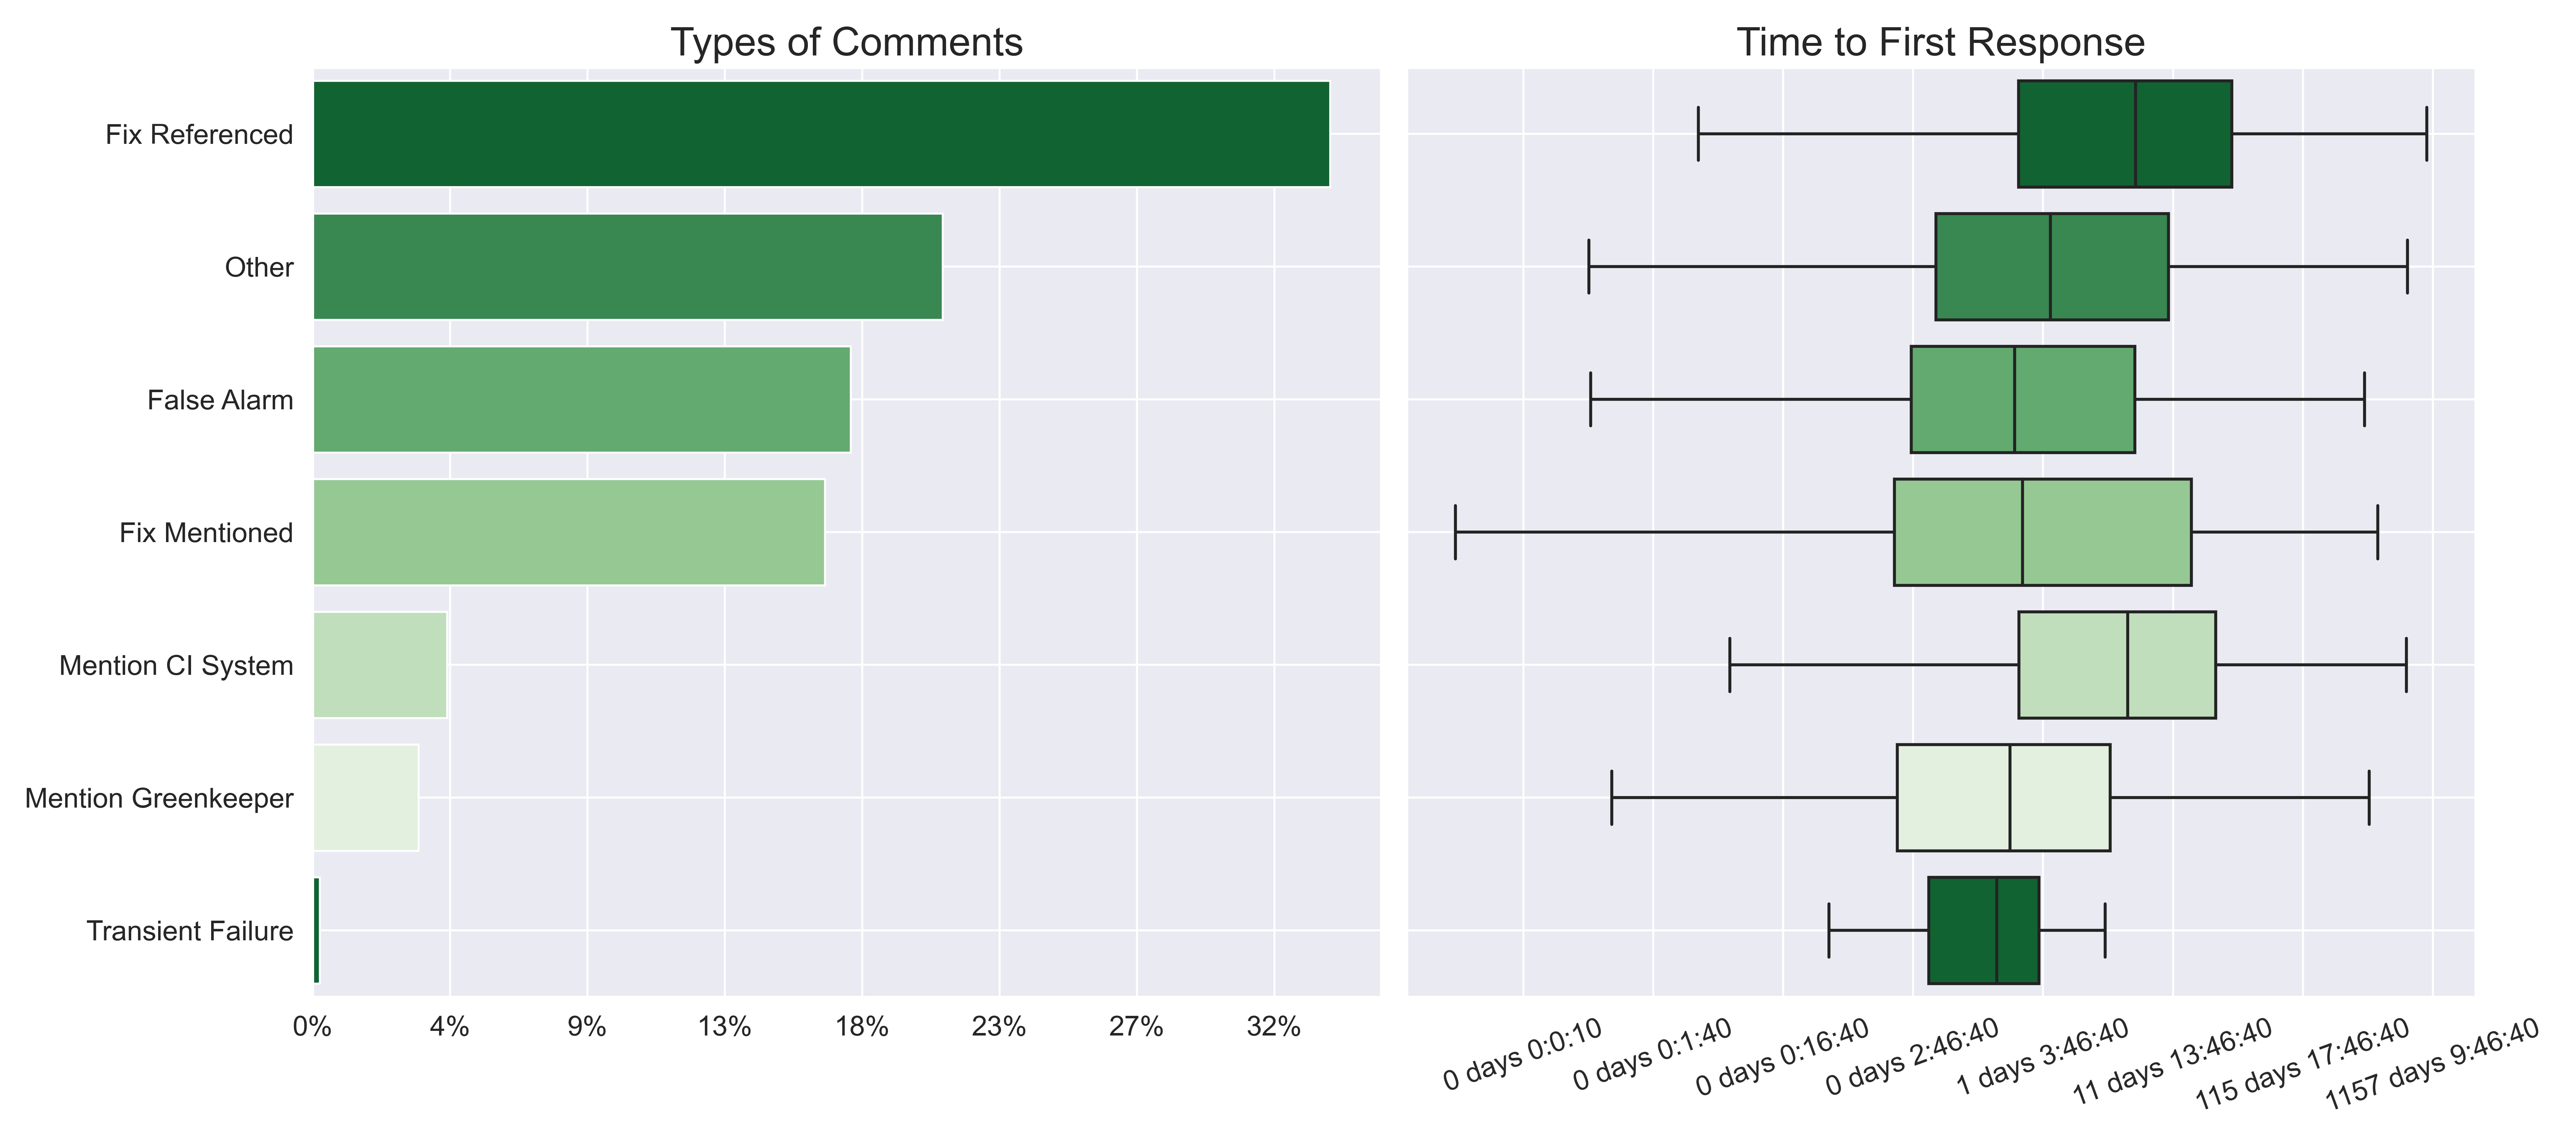
\includegraphics[width=16cm]{images/types_of_comments_and_time_until_comment_type.png}
    \caption{Most common types of comments left by users on in-range breaking build issue reports (left) and how long users take to make each response (right) }
    \label{fig:issue_comments}
\end{figure*}
\par
We saw that practitioners were referencing fixes on these issue reports, so we investigated what these fixes entail. We found that 69.7\% of referenced commits include changes the \textit{package.json} file, 28.5\% include changes to the \textit{package-lock.json} file, and 25.6\% include changes to the \textit{yarn.lock} file. These are all files that are used to specify a projects dependencies. The two lock files are automatically generated and so have a relatively high commit churn, with the \textit{package-lock.json} file having a median commit churn of 101 additions and 130 deletions, and the \textit{yarn.lock} having a median commit churn of 44 additions and 59.5 deletions. However, the \textit{package.json} file, which is manually maintained, has a median commit churn of 1 addition and 1 deletion per commit when fixing an in-range breaking build issue. This suggests that, in order to fix their build, users are simply updating their accepted dependency version range, such as pinning the dependency that is failing the build. Figure \ref{fig:changed_files} summarized the most common files changed in referenced commits on in-range breaking build issues, as well as their commit churn. Additionally, these results shows that it is uncommon for clients to modify their source code that uses these dependencies in order to fix their builds.
\begin{figure*}[h]
    \centering
    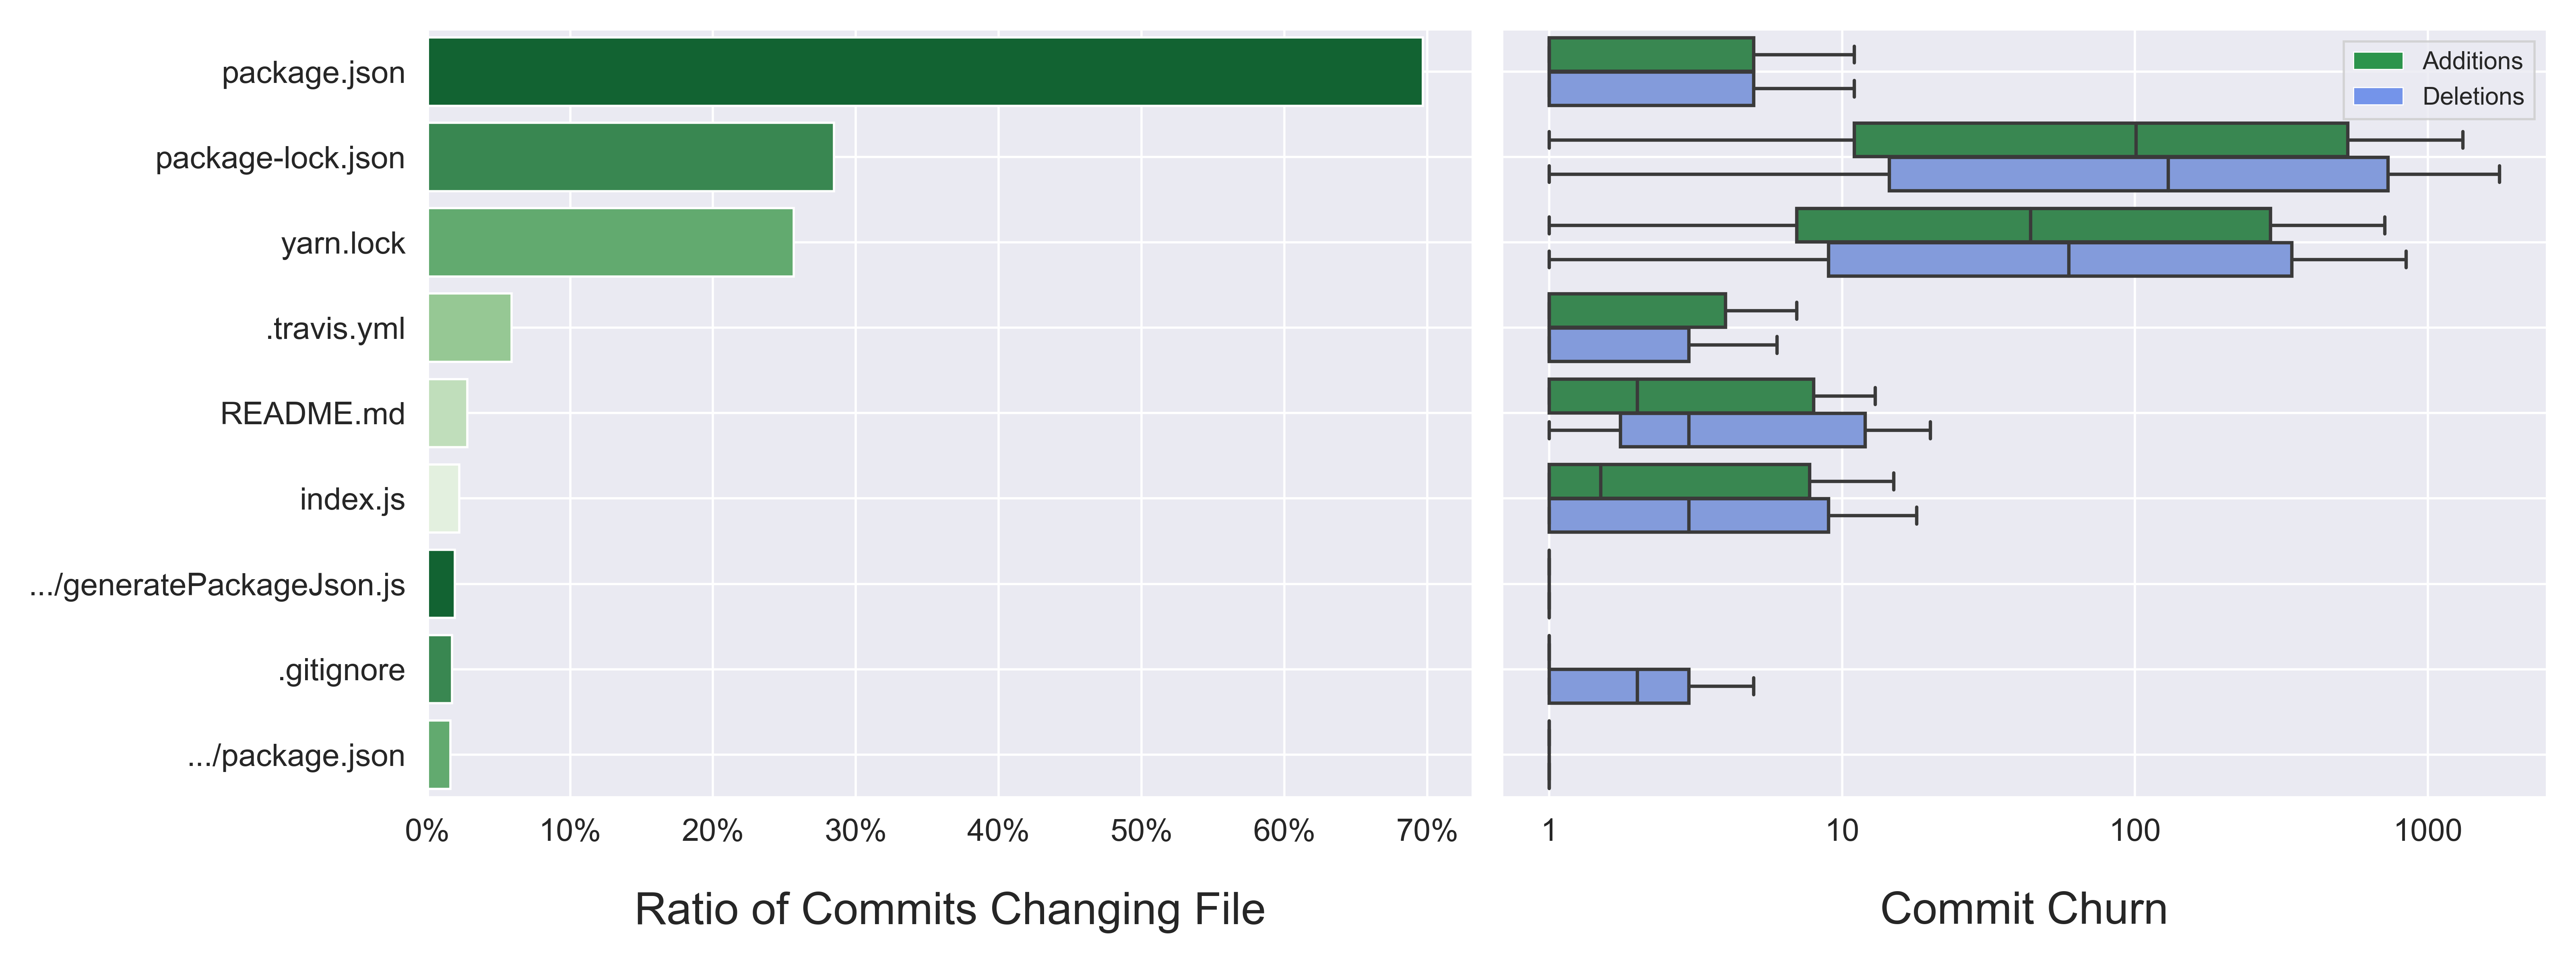
\includegraphics[width=\linewidth]{images/changed_files_ratio_and_commit_churn.png}
    \caption{Most common files changed in commits referenced by in-range breaking build issue reports (left) and the commit churn of each file (right)}
    \label{fig:changed_files}
\end{figure*}
\par
When the Greenkeeper bot opens a breaking build issue report, it will automatically attempt to pin the dependency to the previous version and re-run the build to determine if the issue can be resolved. Pinning a dependency is a legitimate option when developers don’t have the time or resources to fix a problem introduced by a dependency update. Greenkeeper will bundle upgrades for the packages that have to be upgraded together, and it won’t attempt to pin all of the packages in the bundle, which is why 28.1\% of issues don’t have a pin attempt. However, of the issue reports that did have a pin attempt, only 33.1\% resulted in the client's build passing again. This indicates that the majority of these in-range breaking build update issue reports are not actually caused by the dependency being updated. In order to better understand the reasons as to why so many pin attempts fail, we manually analyze a sample of the issue reports that have a failed pin attempt. We found that clients improperly configuring their projects build pipeline was the primary reason for the dependency updates failing, including missing configuration files, invalid credentials, or inconsistent environment versions. We also saw that the builds can fail due to flaky tests, request timeouts, and even  attempting to run the build before the branch had been created in the project repository.
\par
Additionally, we found that Greenkeeper does not take into account the type of error that occurs in the pipeline when testing new dependency updates, and will consider any error that occurs in the pipeline as a build failure. This means that, for example, if a developer that does not conform to the project's linter configuration, then all subsequent builds will fail, and Greenkeeper will open in-range breaking update issue reports for any dependencies that release a new in-range version. If the dependency continues to release new versions, the issue report will become flooded with comments from Greenkeeper confirming that the build is still failing, introducing a lot of noise into projects and distracting from valid issue reports, which practitioners say is one of the main reasons for not using automated dependency management tools \cite{ACM2017_Mirhosseini_AutomatedPullRequests}.
\newline
\par
\fbox{%
    \parbox{8cm}{%
        The majority of client responses mention a fix or confirm the issue is invalid. Most fixes involve small changes to dependency specification files. While pinning the dependency is a legitimate option, it is not as successful as expected due to builds failing for reasons not related to the dependency being updated.
    }%
}